%%%%%%%%%%%%%%%%%%%%%%%%%%%%%%%%%%%%%%%%%%%%%%%%%%%%%%%%%%%%%%%%%%%%%%%%
% Plantilla TFG/TFM
% Escuela Politécnica Superior de la Universidad de Alicante
% Realizado por: Jose Manuel Requena Plens
% Contacto: info@jmrplens.com / Telegram:@jmrplens
%%%%%%%%%%%%%%%%%%%%%%%%%%%%%%%%%%%%%%%%%%%%%%%%%%%%%%%%%%%%%%%%%%%%%%%%

\chapter{Methodology}\label{methodology}

\section{Data}

Our data comprises approximately 400 sessions collected from 80 patients. These
sessions were recorded at various time points and are not uniformly spaced.
Each session's data includes a 3D scan of the patient, along with several
measurements such as weight, height, body fat percentage, etc.

\todo[]{Puedes añadir la tabla que aparece en el paper A Non-Invasive Approach for Total Cholesterol Level Prediction Using Machine Learning}

\todo[]{${https://rua.ua.es/dspace/bitstream/10045/124160/6/Garcia-dUrso_etal_2022_IEEEAccess.pdf}$}

However, the data requires cleaning before usage. Some sessions lack certain
measurements, and there are numerous outliers within the data. After cleaning,
we utilized about 200 sessions.

\todo[]{Puedes añadir un sub-punto hablando del preprocesado de los datos}

\section{Body representation}

In order to represent the body shape we opted to use \gls{smpl}. \gls{smpl}
encodes the body shape and pose using a low-dimensional linear space. The body
shape is encoded using 10 shape parameters ($\beta$), and the pose is encoded
using 72 pose parameters ($\theta$). As our interest lies in body shape, we
employed only the shape parameters.

\def\betaVar{3}
\def\imgWidth{0.3\textwidth}
\def\betaWidth{\textwidth}

\begin{figure}[ht!]
    \centering
    \begin{minipage}[b]{\textwidth}
        \centering
        \includegraphics[width=\imgWidth]{files/visualize_betas/beta_0_-\betaVar_m}
        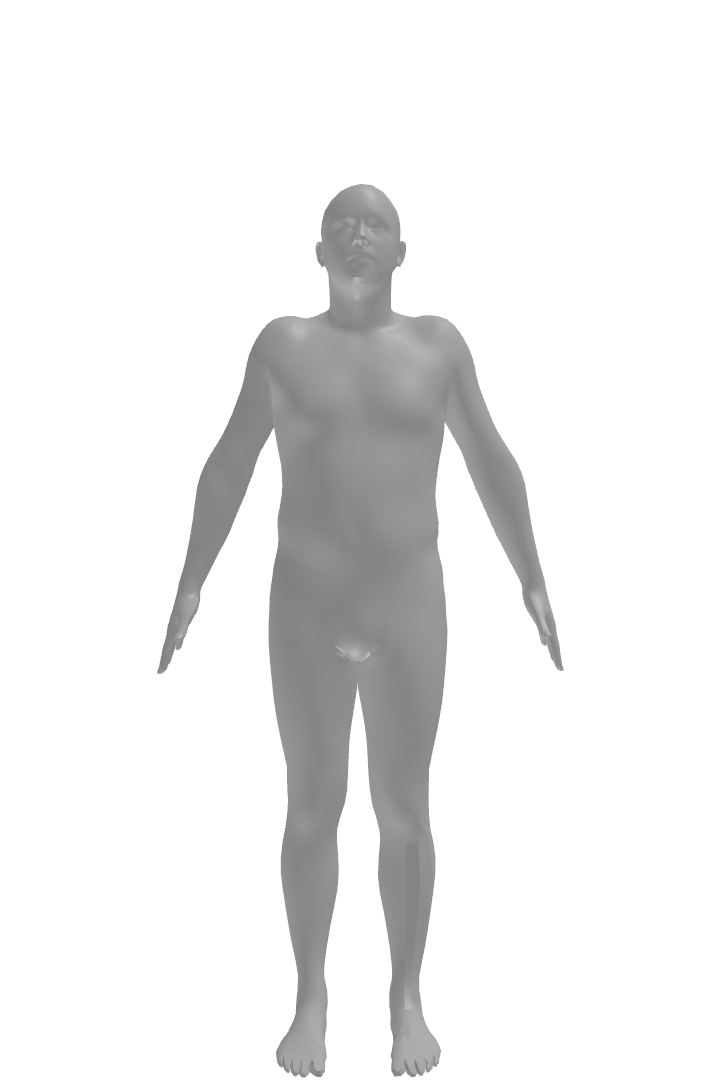
\includegraphics[width=\imgWidth]{files/visualize_betas/baseline_m}
        \includegraphics[width=\imgWidth]{files/visualize_betas/beta_0_\betaVar_m}
        \linebreak
        \includegraphics[width=\imgWidth]{files/visualize_betas/beta_0_-\betaVar_f}
        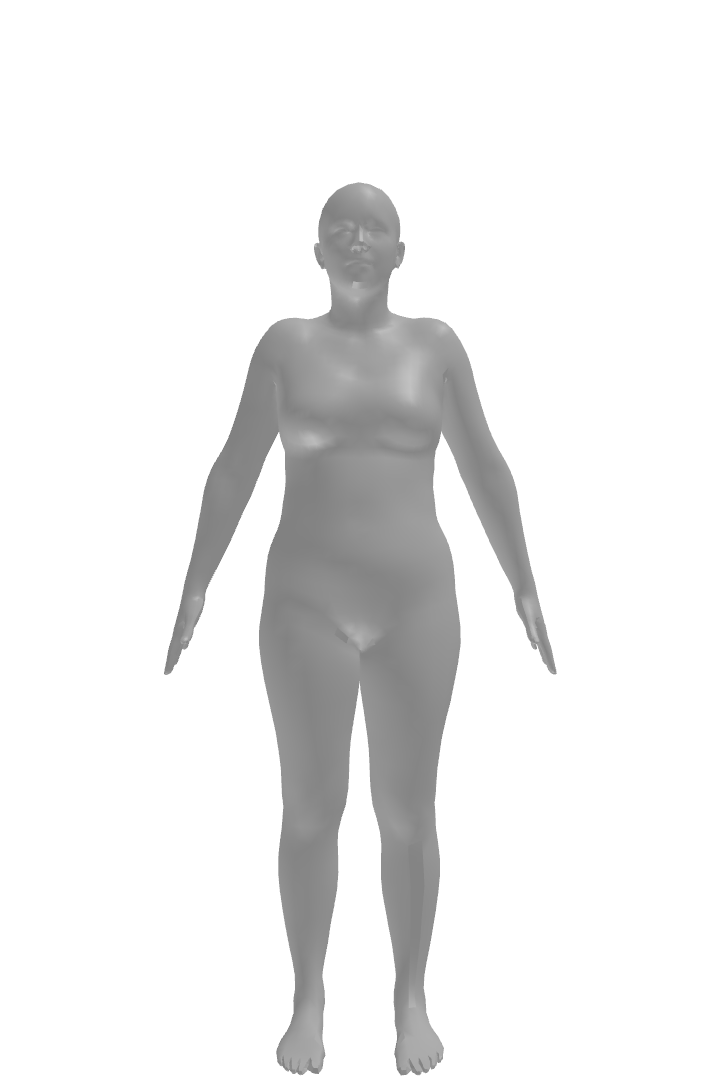
\includegraphics[width=\imgWidth]{files/visualize_betas/baseline_f}
        \includegraphics[width=\imgWidth]{files/visualize_betas/beta_0_\betaVar_f}
        \caption[Effect of varying $\beta_1$ in SMPL.]{$\beta_1 = [-\betaVar, 0, +\betaVar]$.}
        \label{fig:beta-1-vis}
    \end{minipage}
\end{figure}

\begin{figure}[ht!]
    \centering

    \begin{minipage}[b]{\textwidth}
        \centering
        \includegraphics[width=\imgWidth]{files/visualize_betas/beta_1_-\betaVar_m}
        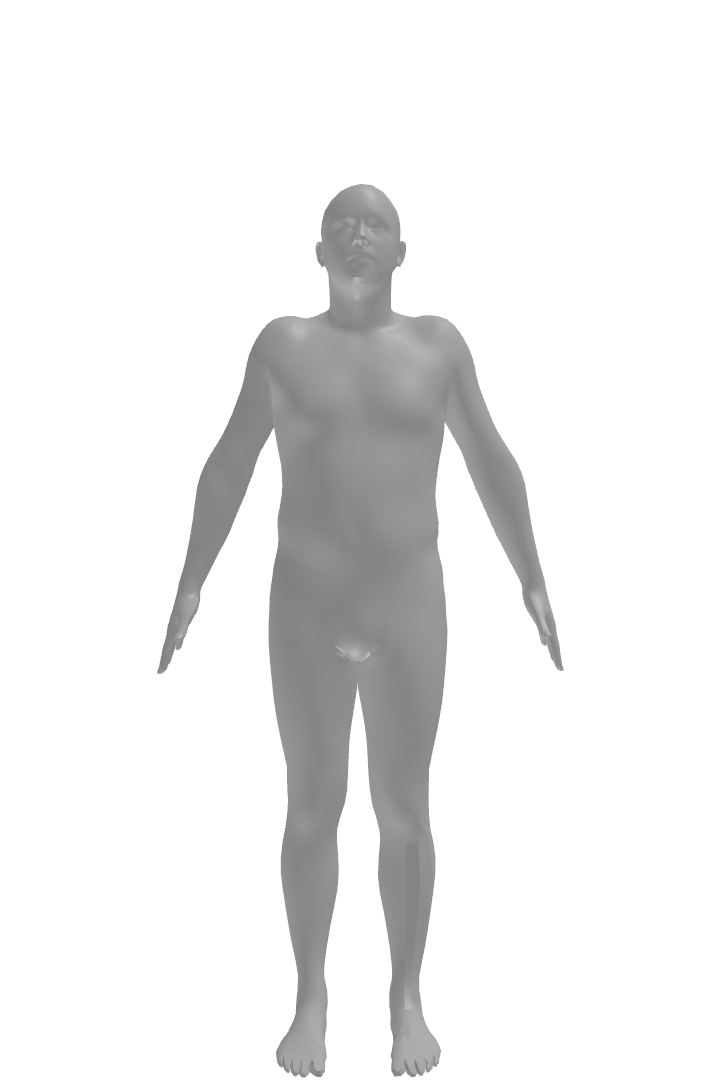
\includegraphics[width=\imgWidth]{files/visualize_betas/baseline_m}
        \includegraphics[width=\imgWidth]{files/visualize_betas/beta_1_\betaVar_m}
        \linebreak
        \includegraphics[width=\imgWidth]{files/visualize_betas/beta_1_-\betaVar_f}
        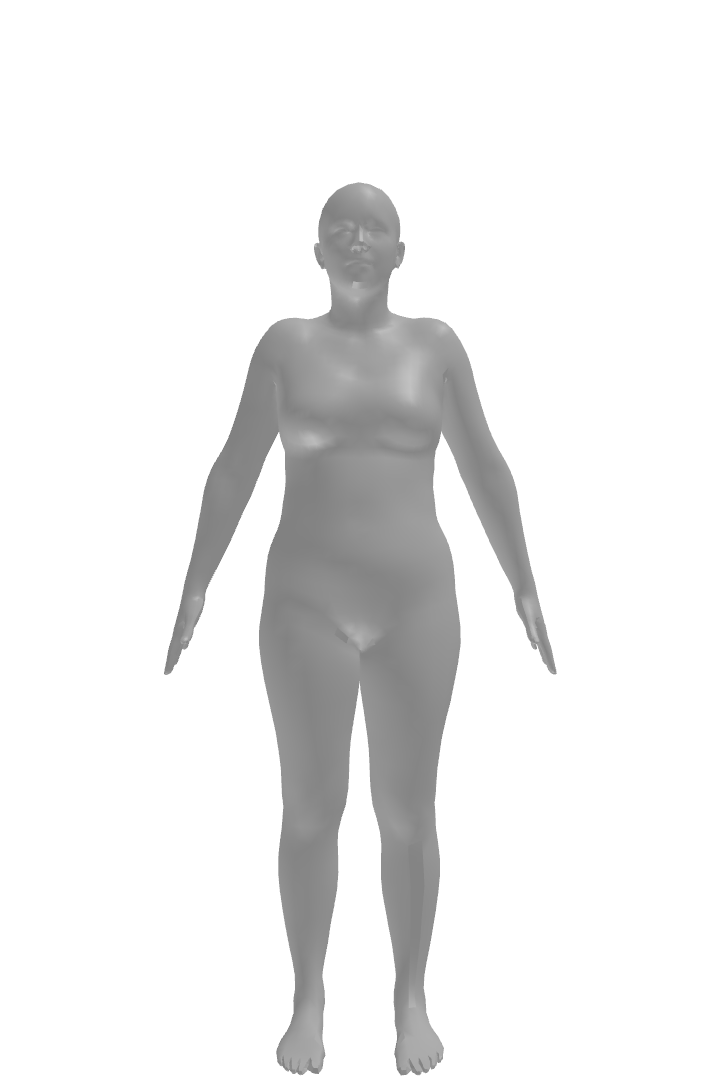
\includegraphics[width=\imgWidth]{files/visualize_betas/baseline_f}
        \includegraphics[width=\imgWidth]{files/visualize_betas/beta_1_\betaVar_f}
        \caption[Effect of varying $\beta_2$ in SMPL.]{$\beta_2 = [-\betaVar, 0, +\betaVar]$.}
    \end{minipage}
\end{figure}

\begin{figure}[ht!]
    \centering

    \begin{minipage}[b]{\textwidth}
        \centering
        \includegraphics[width=\imgWidth]{files/visualize_betas/beta_2_-\betaVar_m}
        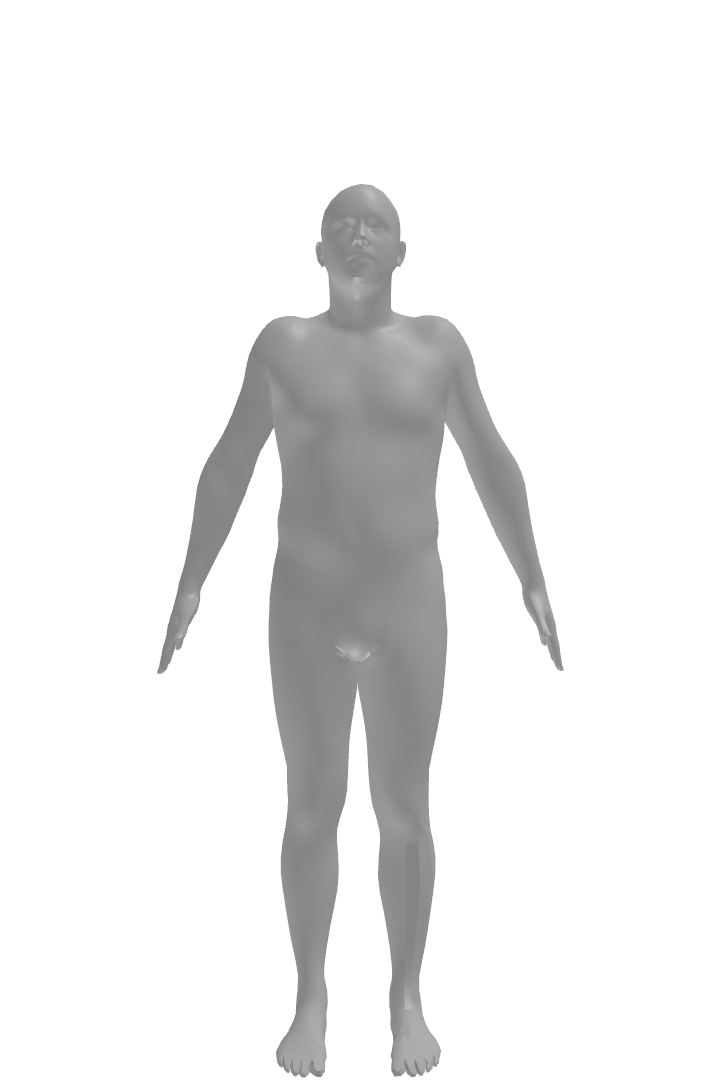
\includegraphics[width=\imgWidth]{files/visualize_betas/baseline_m}
        \includegraphics[width=\imgWidth]{files/visualize_betas/beta_2_\betaVar_m}
        \linebreak
        \includegraphics[width=\imgWidth]{files/visualize_betas/beta_2_-\betaVar_f}
        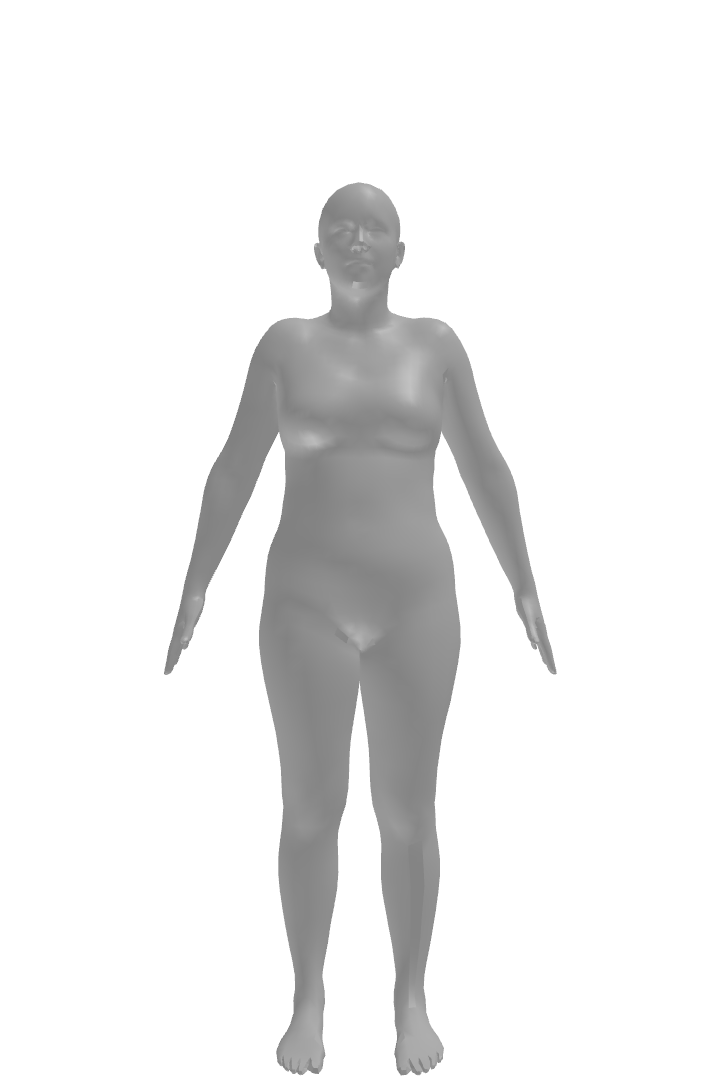
\includegraphics[width=\imgWidth]{files/visualize_betas/baseline_f}
        \includegraphics[width=\imgWidth]{files/visualize_betas/beta_2_\betaVar_f}
        \caption[Effect of varying $\beta_3$ in SMPL.]{$\beta_3 = [-\betaVar, 0, +\betaVar]$.}
    \end{minipage}
\end{figure}

\begin{figure}[ht!]
    \centering

    \begin{minipage}[b]{\textwidth}
        \centering
        \includegraphics[width=\imgWidth]{files/visualize_betas/beta_3_-\betaVar_m}
        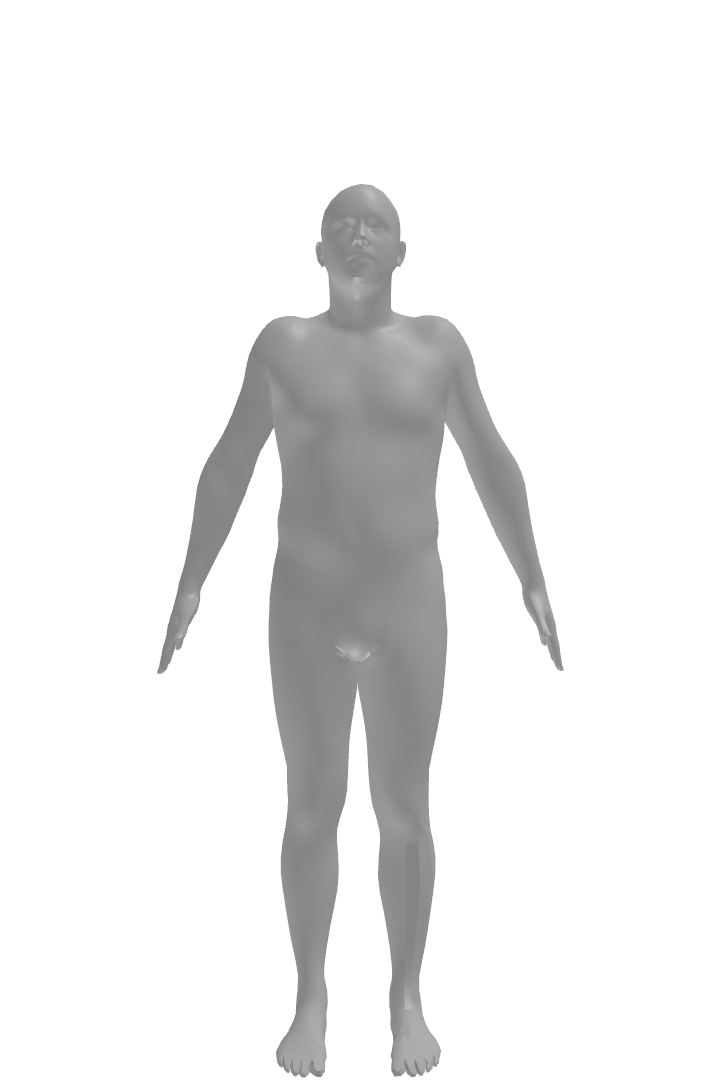
\includegraphics[width=\imgWidth]{files/visualize_betas/baseline_m}
        \includegraphics[width=\imgWidth]{files/visualize_betas/beta_3_\betaVar_m}
        \linebreak
        \includegraphics[width=\imgWidth]{files/visualize_betas/beta_3_-\betaVar_f}
        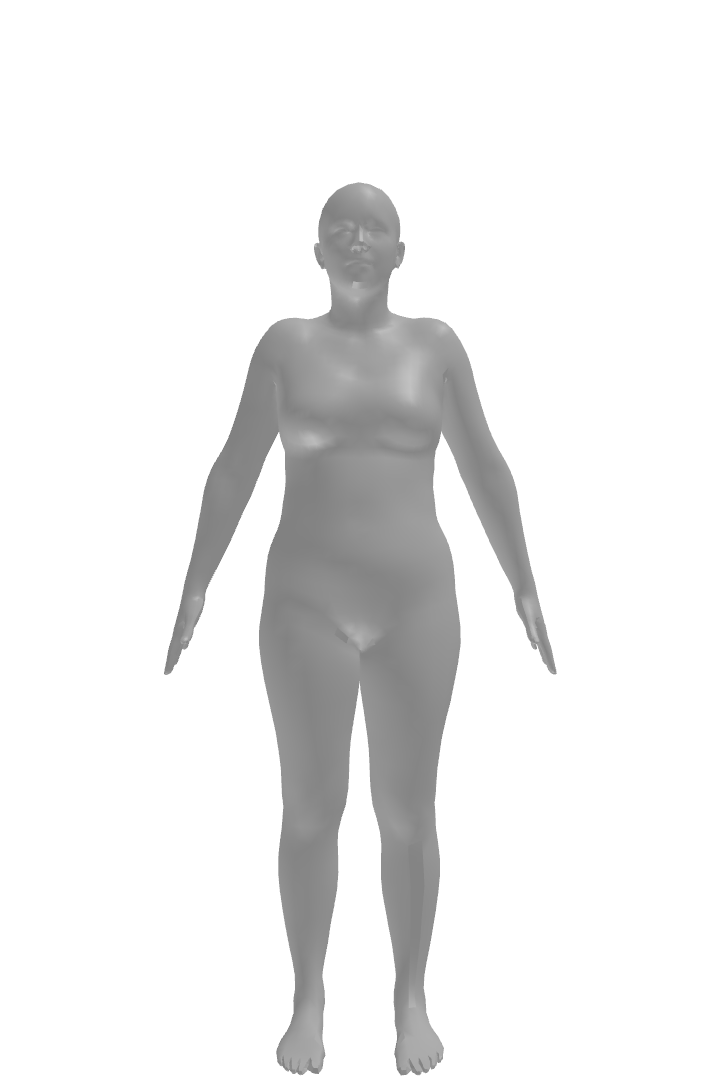
\includegraphics[width=\imgWidth]{files/visualize_betas/baseline_f}
        \includegraphics[width=\imgWidth]{files/visualize_betas/beta_3_\betaVar_f}
        \caption[Effect of varying $\beta_4$ in SMPL.]{$\beta_4 = [-\betaVar, 0, +\betaVar]$.}
    \end{minipage}
\end{figure}

\begin{figure}[ht!]
    \centering

    \begin{minipage}[b]{\textwidth}
        \centering
        \includegraphics[width=\imgWidth]{files/visualize_betas/beta_4_-\betaVar_m}
        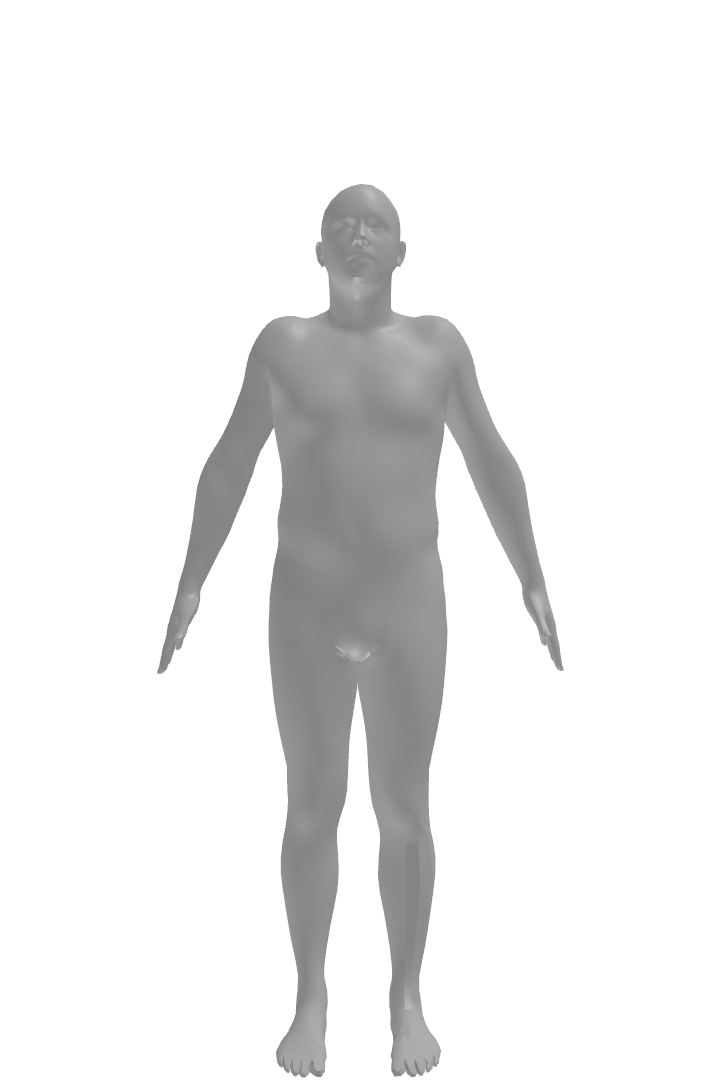
\includegraphics[width=\imgWidth]{files/visualize_betas/baseline_m}
        \includegraphics[width=\imgWidth]{files/visualize_betas/beta_4_\betaVar_m}
        \linebreak
        \includegraphics[width=\imgWidth]{files/visualize_betas/beta_4_-\betaVar_f}
        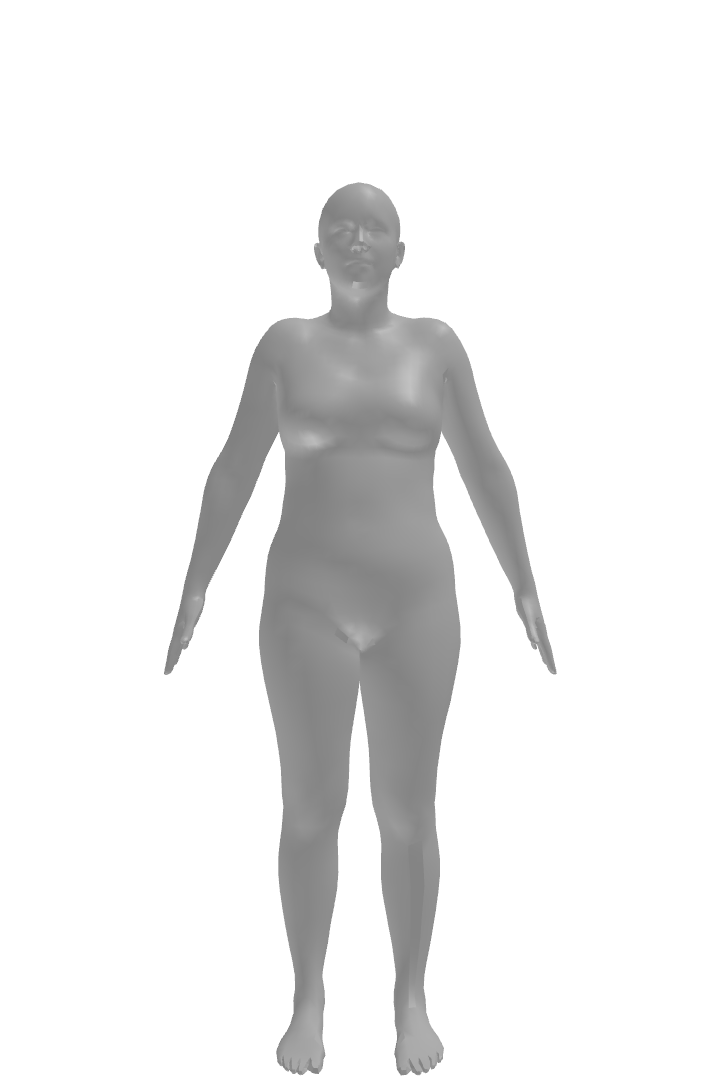
\includegraphics[width=\imgWidth]{files/visualize_betas/baseline_f}
        \includegraphics[width=\imgWidth]{files/visualize_betas/beta_4_\betaVar_f}
        \caption[Effect of varying $\beta_5$ in SMPL.]{$\beta_5 = [-\betaVar, 0, +\betaVar]$.}
    \end{minipage}
\end{figure}

\begin{figure}[ht!]
    \centering

    \begin{minipage}[b]{\textwidth}
        \centering
        \includegraphics[width=\imgWidth]{files/visualize_betas/beta_5_-\betaVar_m}
        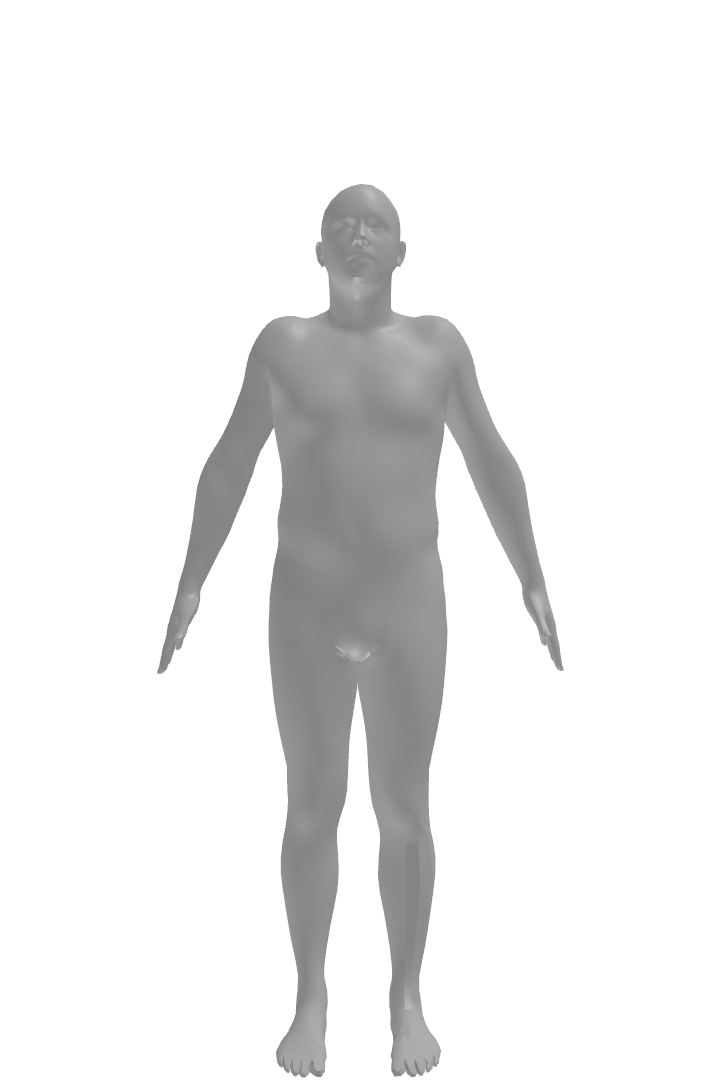
\includegraphics[width=\imgWidth]{files/visualize_betas/baseline_m}
        \includegraphics[width=\imgWidth]{files/visualize_betas/beta_5_\betaVar_m}
        \linebreak
        \includegraphics[width=\imgWidth]{files/visualize_betas/beta_5_-\betaVar_f}
        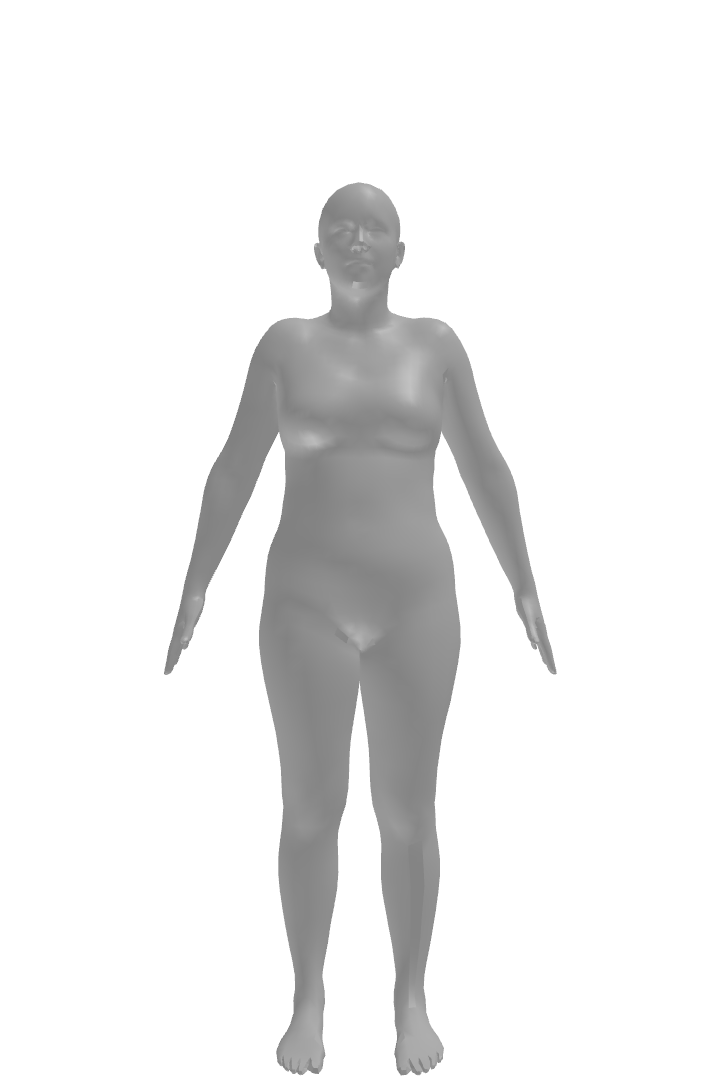
\includegraphics[width=\imgWidth]{files/visualize_betas/baseline_f}
        \includegraphics[width=\imgWidth]{files/visualize_betas/beta_5_\betaVar_f}
        \caption[Effect of varying $\beta_6$ in SMPL.]{$\beta_6 = [-\betaVar, 0, +\betaVar]$.}
    \end{minipage}
\end{figure}

\begin{figure}[ht!]
    \centering

    \begin{minipage}[b]{\textwidth}
        \centering
        \includegraphics[width=\imgWidth]{files/visualize_betas/beta_6_-\betaVar_m}
        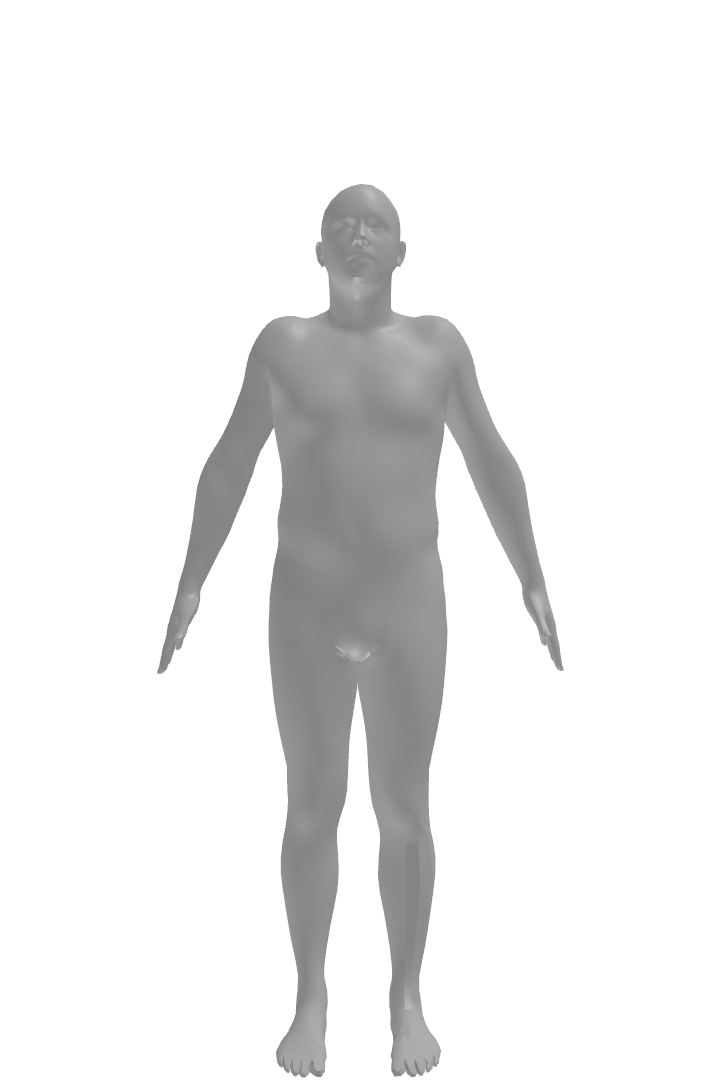
\includegraphics[width=\imgWidth]{files/visualize_betas/baseline_m}
        \includegraphics[width=\imgWidth]{files/visualize_betas/beta_6_\betaVar_m}
        \linebreak
        \includegraphics[width=\imgWidth]{files/visualize_betas/beta_6_-\betaVar_f}
        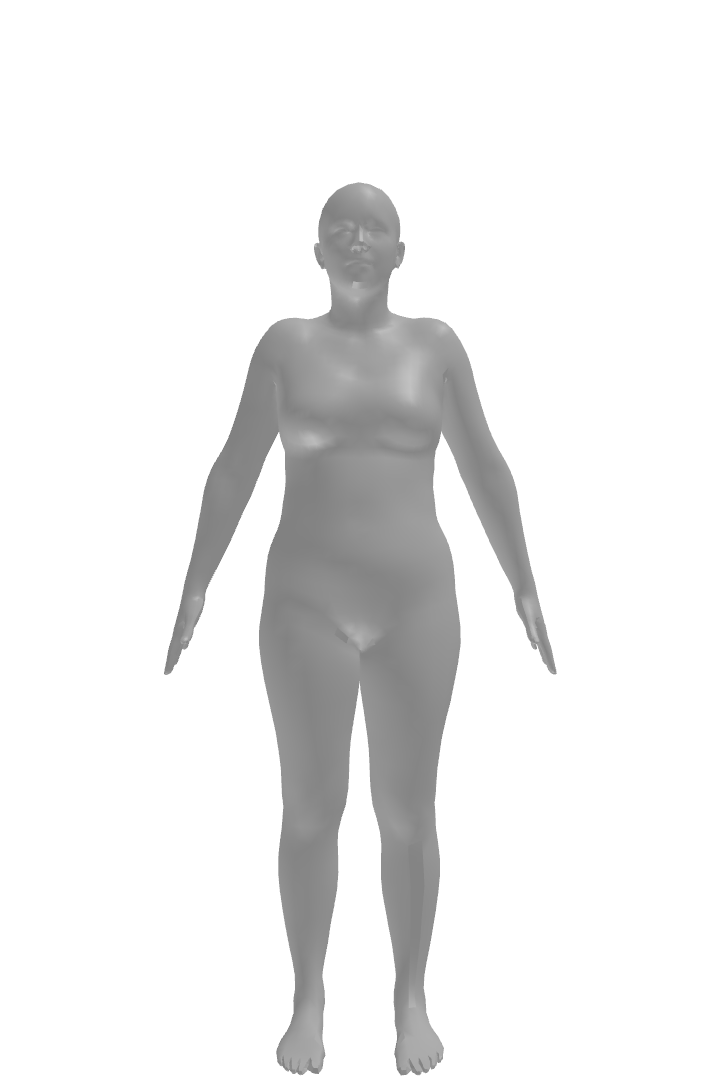
\includegraphics[width=\imgWidth]{files/visualize_betas/baseline_f}
        \includegraphics[width=\imgWidth]{files/visualize_betas/beta_6_\betaVar_f}
        \caption[Effect of varying $\beta_7$ in SMPL.]{$\beta_7 = [-\betaVar, 0, +\betaVar]$.}
    \end{minipage}
\end{figure}

\begin{figure}[ht!]
    \centering

    \begin{minipage}[b]{\textwidth}
        \centering
        \includegraphics[width=\imgWidth]{files/visualize_betas/beta_7_-\betaVar_m}
        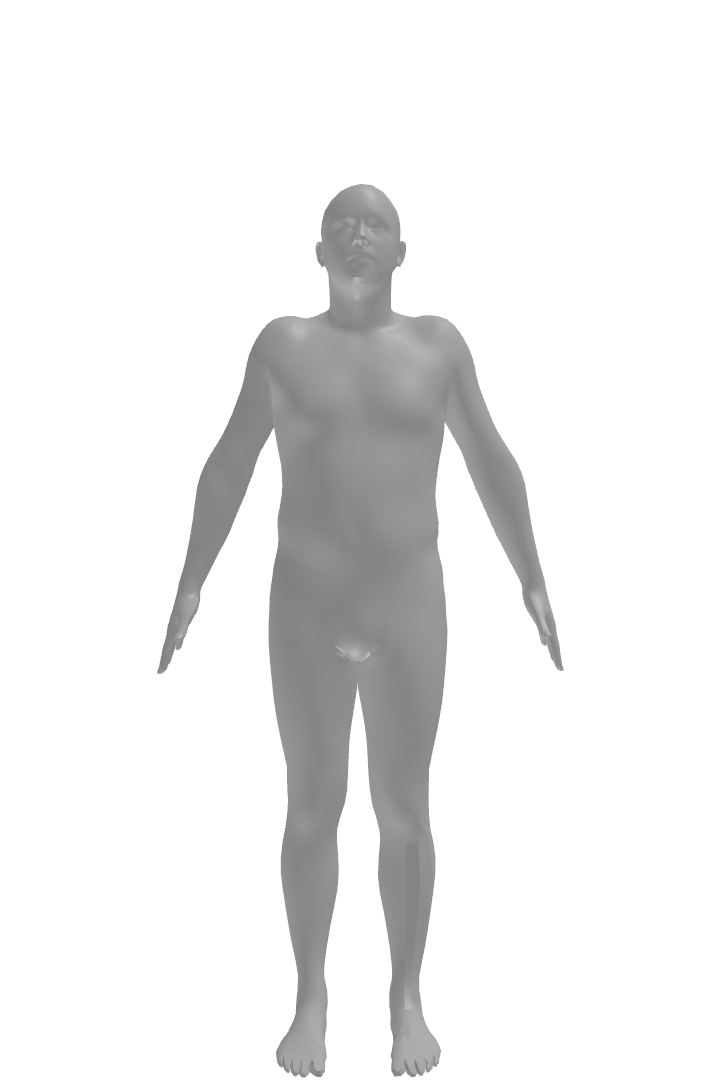
\includegraphics[width=\imgWidth]{files/visualize_betas/baseline_m}
        \includegraphics[width=\imgWidth]{files/visualize_betas/beta_7_\betaVar_m}
        \linebreak
        \includegraphics[width=\imgWidth]{files/visualize_betas/beta_7_-\betaVar_f}
        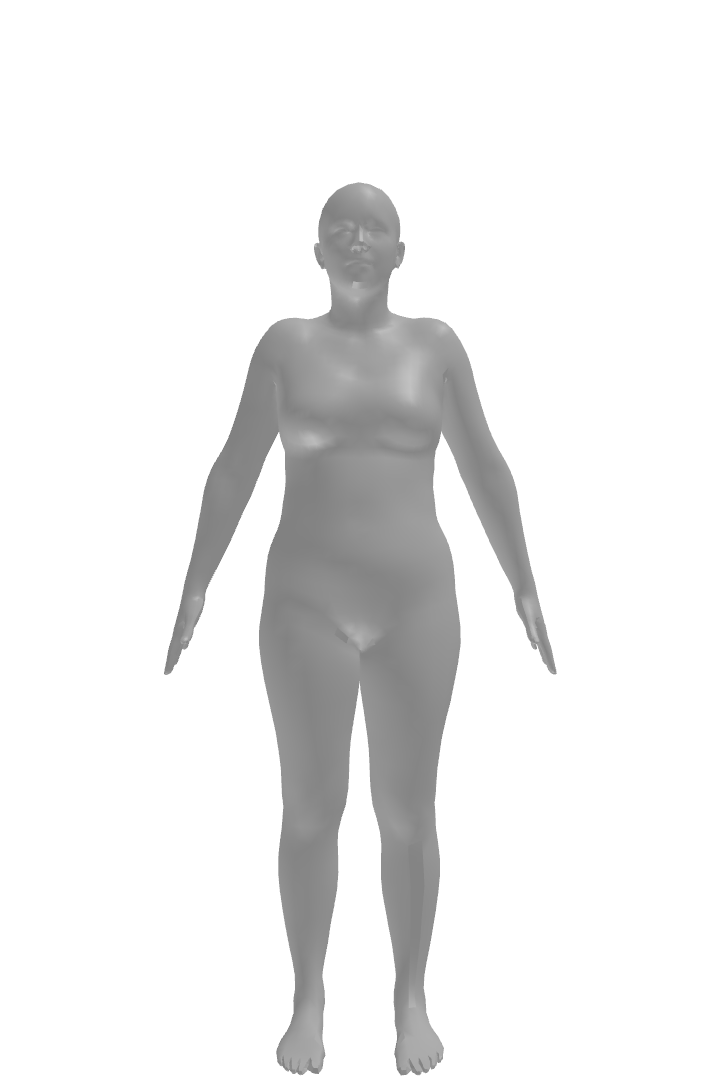
\includegraphics[width=\imgWidth]{files/visualize_betas/baseline_f}
        \includegraphics[width=\imgWidth]{files/visualize_betas/beta_7_\betaVar_f}
        \caption[Effect of varying $\beta_8$ in SMPL.]{$\beta_8 = [-\betaVar, 0, +\betaVar]$.}
    \end{minipage}
\end{figure}

\begin{figure}[ht!]
    \centering

    \begin{minipage}[b]{\textwidth}
        \centering
        \includegraphics[width=\imgWidth]{files/visualize_betas/beta_8_-\betaVar_m}
        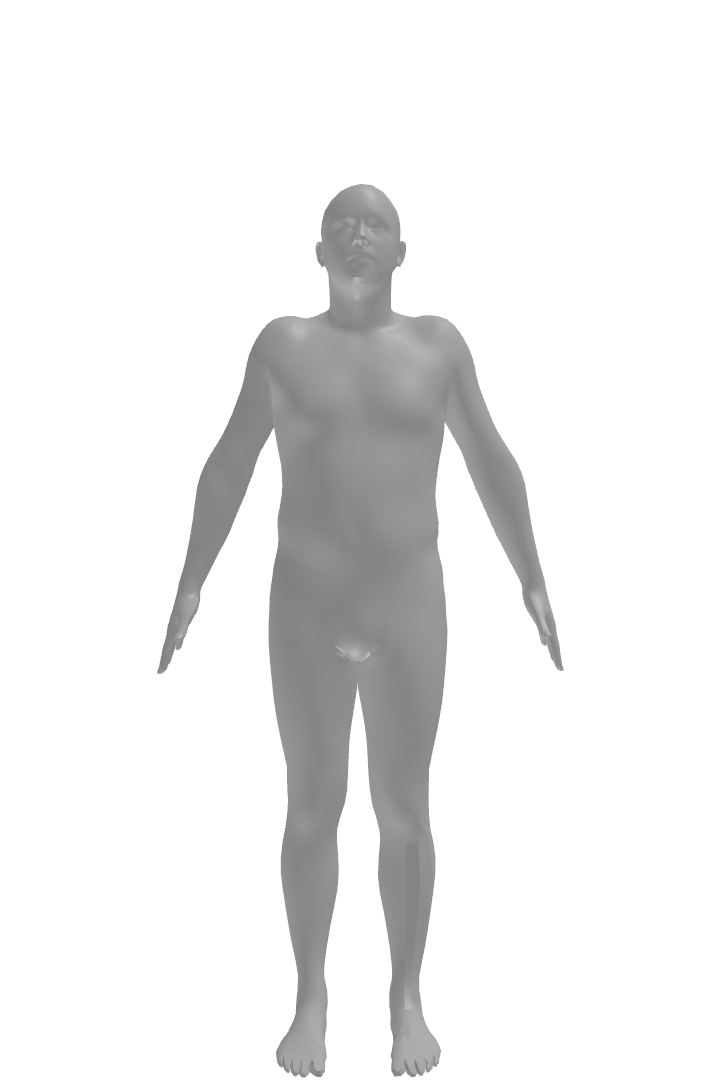
\includegraphics[width=\imgWidth]{files/visualize_betas/baseline_m}
        \includegraphics[width=\imgWidth]{files/visualize_betas/beta_8_\betaVar_m}
        \linebreak
        \includegraphics[width=\imgWidth]{files/visualize_betas/beta_8_-\betaVar_f}
        \includegraphics[width=\imgWidth]{files/visualize_betas/baseline_f}
        \includegraphics[width=\imgWidth]{files/visualize_betas/beta_8_\betaVar_f}
        \caption[Effect of varying $\beta_9$ in SMPL.]{$\beta_9 = [-\betaVar, 0, +\betaVar]$.}
    \end{minipage}
\end{figure}

\begin{figure}[ht!]
    \centering

    \begin{minipage}[b]{\textwidth}
        \centering
        \includegraphics[width=\imgWidth]{files/visualize_betas/beta_9_-\betaVar_m}
        \includegraphics[width=\imgWidth]{files/visualize_betas/baseline_m}
        \includegraphics[width=\imgWidth]{files/visualize_betas/beta_9_\betaVar_m}
        \linebreak
        \includegraphics[width=\imgWidth]{files/visualize_betas/beta_9_-\betaVar_f}
        \includegraphics[width=\imgWidth]{files/visualize_betas/baseline_f}
        \includegraphics[width=\imgWidth]{files/visualize_betas/beta_9_\betaVar_f}
        \caption[Effect of varying $\beta_{10}$ in SMPL.]{$\beta_{10} = [-\betaVar, 0, +\betaVar]$.}
        \label{fig:beta-10-vis}
    \end{minipage}
\end{figure}


Figure~\ref{fig:beta-vis} shows the effect of varying the shape parameters. We
have used a scale of 3 to better show their effect, but in practice the values
are much smaller. $\beta_0$ controls the overall height of the body, while
$\beta_1$ has a large correlation with the body mass index.

\begin{table}[h]
    \centering
    \begin{tabular}{ |c|c|c|c|c|c|c|c|c|c|c| }
        \hline
             & $\beta_1$ & $\beta_2$ & $\beta_3$ & $\beta_4$ & $\beta_5$ & $\beta_6$ & $\beta_7$ & $\beta_8$ & $\beta_9$ & $\beta_{10}$ \\
        \hline
        mean & 0.88      & -0.73     & 0.34      & 0.01      & 0.06      & 0.06      & 0.11      & 0.02      & 0.01      & 0.11         \\
        \hline
        std  & 0.97      & 0.78      & 0.26      & 0.21      & 0.12      & 0.13      & 0.08      & 0.03      & 0.03      & 0.08         \\
        \hline
        min  & -1.42     & -2.57     & -0.64     & -0.65     & -0.23     & -0.25     & -0.14     & -0.07     & -0.08     & -0.17        \\
        \hline
        25\% & 0.12      & -1.26     & 0.15      & -0.14     & -0.01     & -0.02     & 0.04      & 0.00      & -0.01     & 0.06         \\
        \hline
        50\% & 0.94      & -0.69     & 0.36      & 0.03      & 0.04      & 0.02      & 0.11      & 0.02      & 0.01      & 0.11         \\
        \hline
        75\% & 1.66      & -0.20     & 0.52      & 0.17      & 0.14      & 0.14      & 0.16      & 0.04      & 0.04      & 0.17         \\
        \hline
        max  & 2.90      & 2.96      & 0.97      & 0.45      & 0.39      & 0.47      & 0.36      & 0.13      & 0.16      & 0.30         \\
        \hline
    \end{tabular}
    \caption{Statistics of the shape parameters}
\end{table}

\section{Neural network architecture}

Given the nature of the data, we decided to use a neural network to predict the
changes in the body shape. Since the data is temporal, we need to use a neural
network architecture that can handle temporal data.

There are different neural network architectures that work well with temporal
data. Recurrent neural networks are a type of neural networks that feed the
output of the previous step as input to the next step. This allows them to
remember information from previous steps, which is useful for time series.
However, they can `forget' information from the beginning of the sequence,
which is a problem known as vanishing gradients. There are some variations of
recurrent neural networks that try to solve this problem, such as \gls{lstm}
and \gls{gru}.

Transformer networks are a relatively new type of neural network that has been
used with great success in natural language processing. They are based on
attention mechanisms, which allow them to focus on specific parts of the input
sequence. This makes them very useful for time series, since they can focus on
the most relevant parts of the sequence. The big disadvantage of transformer
networks for this application is that they require large amounts of training
data\todo[]{citation needed}, which is not available in this case.

We ended up using an neural network architecture that uses an \gls{lstm}.

\section{Training}

\subsection{Variability in the dates of the sessions}

The dataset's sessions are not uniformly spaced in time, varying from a few
days to several months apart. To mitigate this issue, we:

Calculated a variable representing the number of days until the next session.

Modified the neural network to predict the daily change in variables, instead
of predicting the variables for the following session.

We implemented a residual connection to the neural network, enabling it to
predict the change in variables from one session to the next. Then, we
multiplied this change by the number of days until the next session and added
it to the previous session to calculate the predicted values for the next
session. This approach assumes a linear change between sessions—an
approximation suited to our purpose. We augmented the data by randomly removing
intermediate sessions and recalculating the number of days until the next
session.

\section{Evaluation}

\section{Results}